\chapter{Metodologia}
\label{ch:identificador}
	\begin{resumocapitulo}
		Este capítulo detalha as metodologias empregadas na análise do consumo de café no Brasil com o uso de machine learning, enfatizando as bibliotecas de Python: Pandas, Matplotlib e Seaborn. Pandas facilita a análise de dados com configurações personalizáveis que aumentam a produtividade (Voitto, 2021). Matplotlib é utilizada para criar gráficos e visualizações de dados (Medium, 2020). Seaborn melhora a estética dos gráficos, tornando-os mais sofisticados e claros (Voooo, 2017). Essas ferramentas são essenciais para manipulação eficaz dos dados e geração de insights.
	\end{resumocapitulo}

	\section{Visão Geral}
			Essas metodologias são essenciais para uma análise aprofundada do consumo de café no Brasil, permitindo a manipulação eficiente dos dados e a aplicação de técnicas avançadas de machine learning para gerar insights valiosos.

   
	\section{CONFIGURANDO A TABELA QUE SERÁ UTILIZADA}
	\label{sec:identificao}
\label{sec:figura}
A Figura~\ref{figuras/configuraçao-introduçao.png} demostra como foi feito a configuração para ser instalada.
\begin{figure}[!ht]
	{\centering
		\caption{Descrição da figura.}
		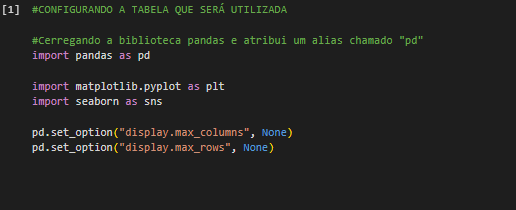
\includegraphics[width=1.0\textwidth]{figuras/configuraçao-introduçao.png}
		\label{figuras/configuraçao-introduçao.png}
		\fonte{Google Colab}
	}
\end{figure} \\ \\ \\ \\ \\ \\ \\ 

\section{Realizando a conexão com o google Drive}
	\label{sec:identificao}
\label{sec:figura}
A Figura~\ref{figuras/configuraçao- resumo.png} demostra como foi feito a conexão com o Google Dive.
\begin{figure}[!ht]
\begin{figure}
	\end{figure}
		{\centering
		\caption{Descrição da figura.}
		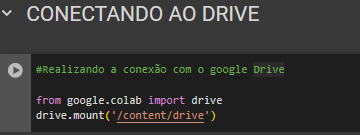
\includegraphics[width=1.0\textwidth]{figuras/configuraçao- resumo.png}
		\label{figuras/configuraçao- resumo.png}
		\fonte{Google Colab}
	}
\end{figure} \\ \\ \\ \\ \\ \\ \\ \\ \\ \\ \\ \\ \\ \\ \\ 

\section{IMPORTANDO DADOS DO BANCO}
	\label{sec:identificao}
\label{sec:figura}
A Figura~\ref{figuras/configuraçao-introduçao.png} demostra como foi feito a importãode Banco de Dados.
\begin{figure}[!ht]
	{\centering
		\caption{Descrição da figura.}
		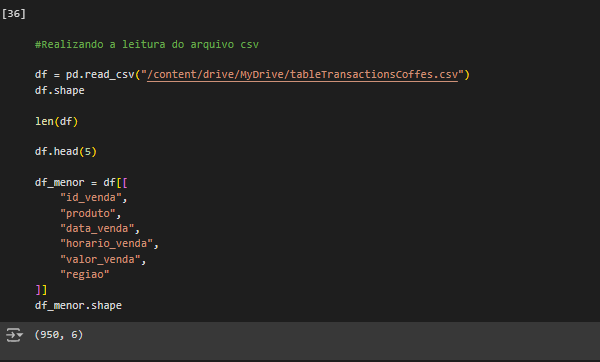
\includegraphics[width=1.0\textwidth]{figuras/configuraçao-dados.png}
		\label{figuras/configuraçao-introduçao.png}
		\fonte{Google Colab}
	}
\end{figure} \\ \\ \\ \\ \\ \\ \\  \\ \\ \\ \\ \\ 


\section{REALIZANDO A CONEXÃO COM O GOOGLE DRIVE    }
	\label{sec:identificao}
\label{sec:figura}
A Figura~\ref{figuras/figuras/cconfiguraçao-.analise-vendas.} demostra como foi feito a conexão com o Googe Drive.
\begin{figure}[!ht]
	{\centering
		\caption{Descrição da figura.}
		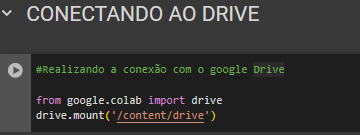
\includegraphics[width=1.0\textwidth]{figuras/configuraçao- resumo.png}
		\label{figuras/figuras/cconfiguraçao-.analise-vendas.}
		\fonte{Google Colab}
	}
\end{figure} \\ \\ \\ \\ \\ \\ \\ \\ \\ \\ \\ \\ \\ \\ \\ \\ \\ \\ \\ \\ \\ 

\section{IMPORTANDO DADOS DO BANCO}
	\label{sec:identificao}
\label{sec:figura}
A Figura~\ref{figuras/figuras/configuraçao-importando-dados-banco.png} demostra como foi feito a importãode Banco de Dados.
\begin{figure}[!ht]
	{\centering
		\caption{Descrição da figura.}
		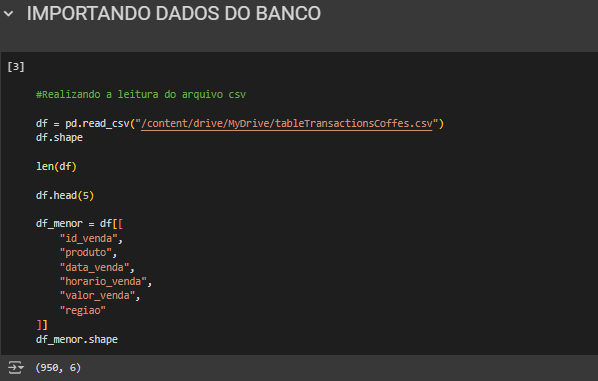
\includegraphics[width=1.0\textwidth]{figuras/configuraçao-importando-dados-banco.png}
		\label{figuras/figuras/configuraçao-importando-dados-banco.png}
		\fonte{Google Colab}
	}
\end{figure} \\ \\ \\ \\ \\ \\ \\  \\ \\ \\ \\ \\ 

\section{ANALISE DE VENDAS DE CAFÉ POR LOJA}
	\label{sec:identificao}
\label{sec:figura}
A Figura~\ref{figuras/figuras/configuraçao-analise-vendas-lojas.png} demostra como foi feito a analise de vendas de café por loja .
\begin{figure}[!ht]
	{\centering
		\caption{Descrição da figura.}
		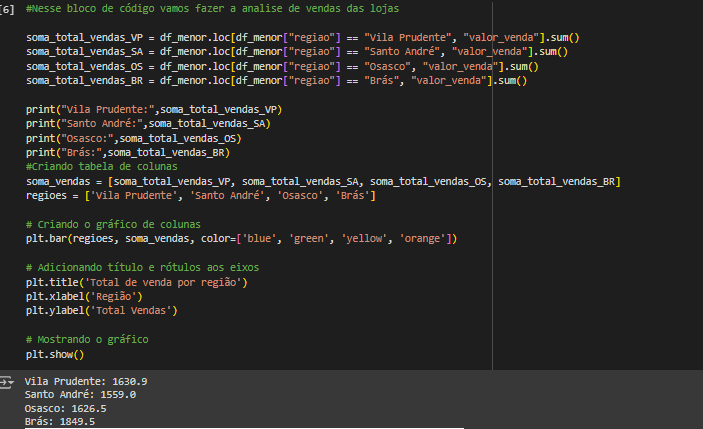
\includegraphics[width=1.0\textwidth]{figuras/configuraçao-analise-vendas-lojas.png}
		\label{figuras/figuras/configuraçao-analise-vendas-lojas.png}
		\fonte{Google Colab}
	}
\end{figure} \\ \\ \\ \\ \\ \\ \\  \\ \\ \\ \\ \\ 

\section{DATAFRAME DOS PRODUTOS MAIS VENDIPOS POR LOJA}
	\label{sec:identificao}
\label{sec:figura}
A Figura~\ref{figuras/figuras/configuraçao-data-freme-vendidos-loja.png} demostra um pequeno Dataframe com os produtos mais vendidos de cada loja .
\begin{figure}[!ht]
	{\centering
		\caption{Descrição da figura.}
		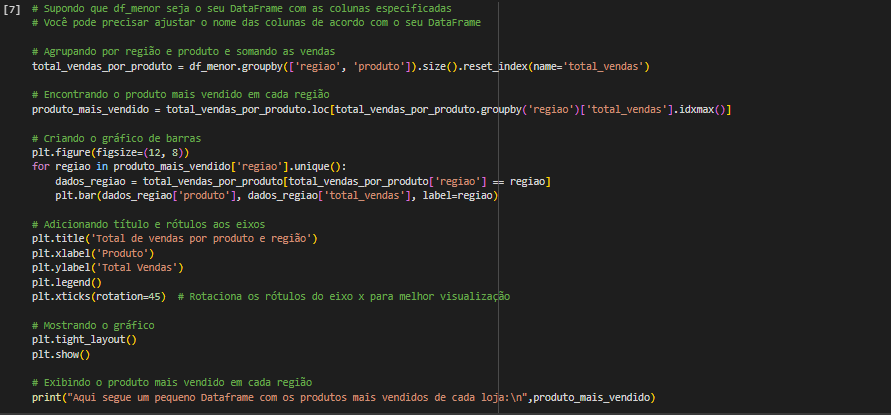
\includegraphics[width=1.0\textwidth]{figuras/configuraçao-data-freme-vendidos-loja.png}
		\label{figuras/figuras/configuraçao-data-freme-vendidos-loja.png}
		\fonte{Google Colab}
	}
\end{figure} \\ \\ \\ \\ \\ \\ \\  \\ \\ \\ \\ \\ \\ \ \\ \\ \\

\section{OPORTUNIDADE DE CRESCIMENTO DE VENDAS}
	\label{sec:identificao}
\label{sec:figura}
A Figura~\ref{figuras/figuras/configuraçao-oportunidade-crescimento.png} demostra um pequeno Dataframe com os produtos mais vendidos de cada loja .
\begin{figure}[!ht]
	{\centering
		\caption{Descrição da figura.}
		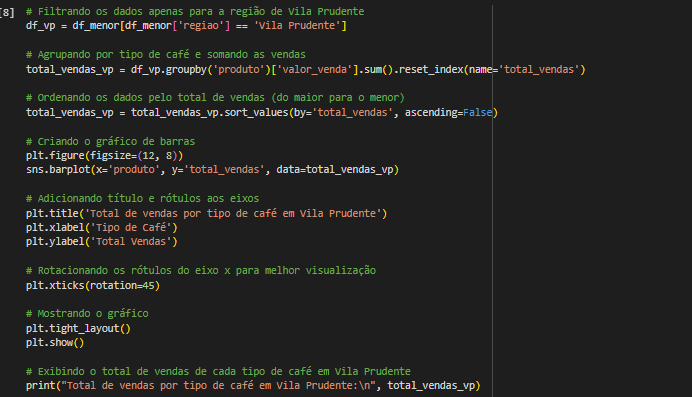
\includegraphics[width=1.0\textwidth]{figuras/configuraçao-oportunidade-crescimento.png}
		\label{figuras/figuras/configuraçao-oportunidade-crescimento.png}
		\fonte{Google Colab}
	}
\end{figure} \\ \\ \\ \\ \\ \\ \\  \\ \\ \\ \\ \\ 

\section{TOTAL DE VENDAS DE CAFÉ NA REGIÃO DE SANTO ANDRÉ}
	\label{sec:identificao}
\label{sec:figura}
A Figura~\ref{figuras/configuraçao-mais-vendidos-Santo-André.png} demostra um total de vendas por tipo de café em Santo André .
\begin{figure}[!ht]
	{\centering
		\caption{Descrição da figura.}
		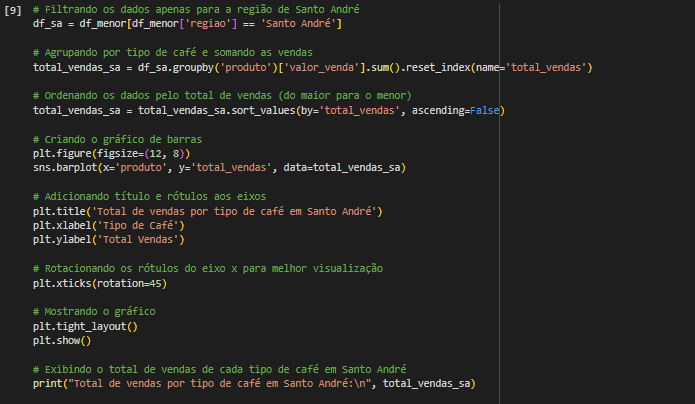
\includegraphics[width=1.0\textwidth]{figuras/configuraçao-mais-vendidos-Santo-André.png}
		\label{figuras/configuraçao-mais-vendidos-Santo-André.png}
		\fonte{Google Colab}
	}
\end{figure} \\ \\ \\ \\ \\ \\ \\  \\ \\ \\ \\ \\ \\ \\ \\ \\

\section{TOTAL DE VENDAS DE CAFÉ NA REGIÃO DE OSASCO}
	\label{sec:identificao}
\label{sec:figura}
A Figura~\ref{figuras/configuraçao-mais-vendido-Osasco.png} demostra um total de vendas por tipo de café na região de Osasco .
\begin{figure}[!ht]
	{\centering
		\caption{Descrição da figura.}
		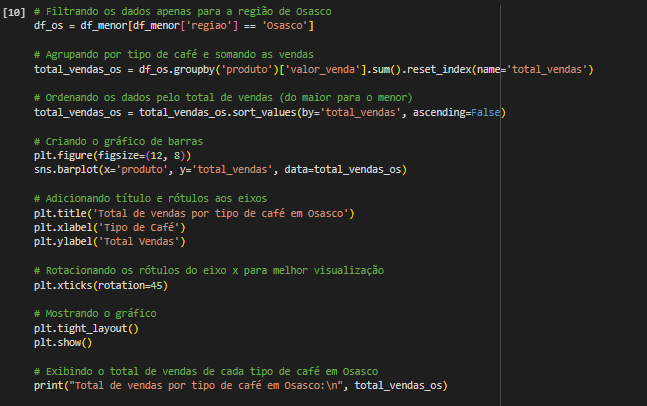
\includegraphics[width=1.0\textwidth]{figuras/configuraçao-mais-vendido-Osasco.png}
		\label{figuras/configuraçao-mais-vendido-Osasco.png}
		\fonte{Google Colab}
	}
\end{figure} \\ \\ \\ \\ \\ \\ \\  \\ \\ \\ \\ \\ 

\section{TOTAL DE VENDAS DE CAFÉ NA REGIÃO DO BRÁS  }
	\label{sec:identificao}
\label{sec:figura}
A Figura~\ref{figuras/configuraçao-mais-vendido-Bras.png} demostra um total de vendas por tipo de café na região do Brás.
\begin{figure}[!ht]
	{\centering
		\caption{Descrição da figura.}
		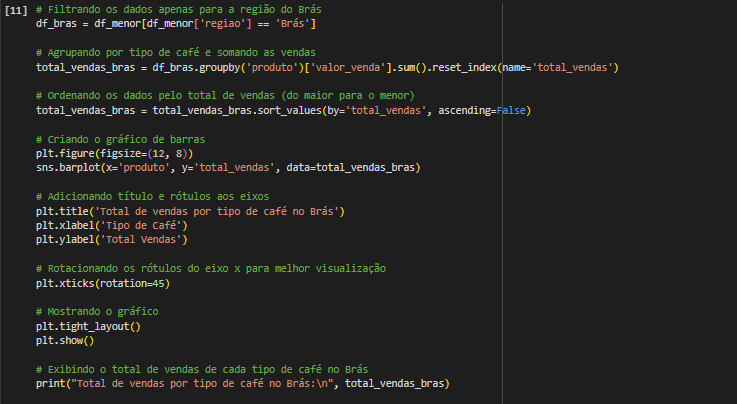
\includegraphics[width=1.0\textwidth]{figuras/configuraçao-mais-vendido-Bras.png}
		\label{figuras/configuraçao-mais-vendido-Bras.png}
		\fonte{Google Colab}
	}
\end{figure} \\ \\ \\ \\ \\ \\ \\  \\ \\ \\ \\ \\ 

\section{FILTRANDO TIPO DE CAFÉ ESPECIFICO PARA UMA ANALISE EXPLORATÓRIA}
	\label{sec:identificao}
\label{sec:figura}
A Figura~\ref{figuras/configuraçao-cafe-expresso-regiao.png} demostra um total de café mais vendido pelo tipo de café expresso por regiões .
\begin{figure}[!ht]
	{\centering
		\caption{Descrição da figura.}
		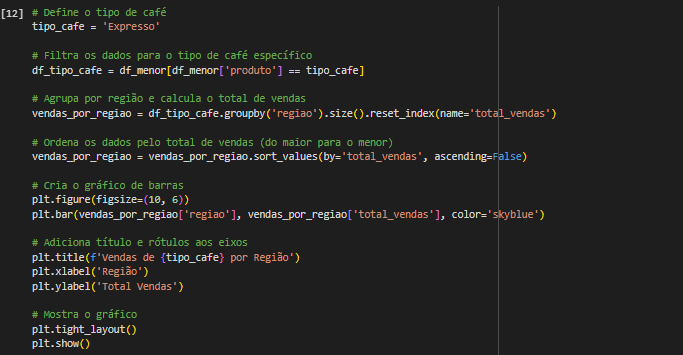
\includegraphics[width=1.0\textwidth]{figuras/configuraçao-cafe-expresso-regiao.png}
		\label{figuras/configuraçao-cafe-expresso-regiao.png}
		\fonte{Google Colab}
	}
\end{figure} \\ \\ \\ \\ \\ \\ \\  \\ \\ \\ \\ \\ 

\section{REALIZANDO O  AGRUPAMENTO DE TODOS OS TIPOS DE CAFÉS E EFETUANDO OS VALORES DE CADA VENDA}
	\label{sec:identificao}
\label{sec:figura}
A Figura~\ref{figuras/configuraçao-somando-todos-cafes-valores-vendas.png} demostra um total de Cafés mais vendidos e quanto renderam.
\begin{figure}[!ht]
	{\centering
		\caption{Descrição da figura.}
		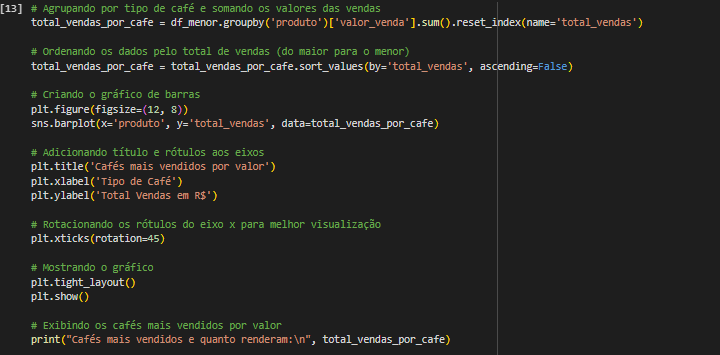
\includegraphics[width=1.0\textwidth]{figuras/configuraçao-somando-todos-cafes-valores-vendas.png}
		\label{figuras/configuraçao-somando-todos-cafes-valores-vendas.png}
		\fonte{Google Colab}
	}
\end{figure} \\ \\ \\ \\ \\ \\ \\  \\ \\ \\ \\ \\ 

\section{CONCLUSÃO DE CAFÉS MAIS VENDIDOS POR VALORES EM CADA REGIÃO}
	\label{sec:identificao}
\label{sec:figura}
A Figura~\ref{ffiguras/configuraçao-resultado-cafes-mais-vendidos-por-regiao-valores.png} demostra uma conclusão em nossa analise exploratória de cafés mais vendidos por valor em cada região.
\begin{figure}[!ht]
	{\centering
		\caption{Descrição da figura.}
		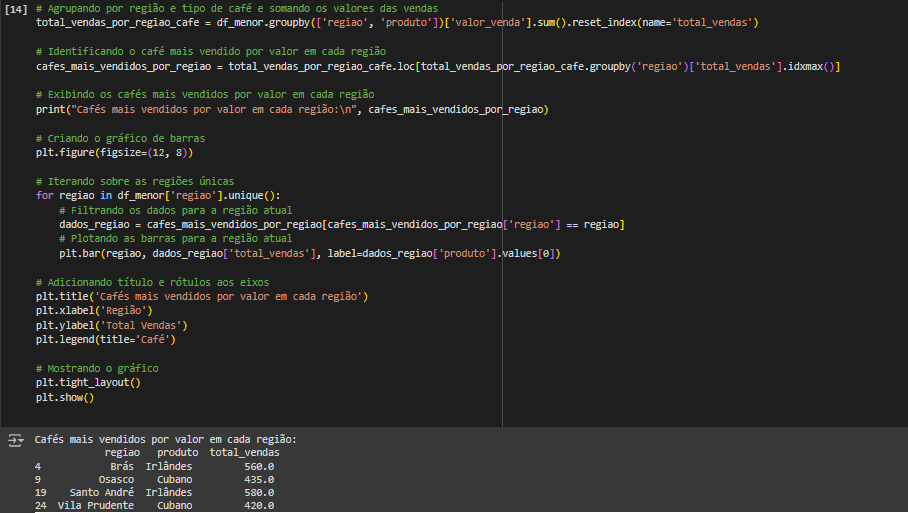
\includegraphics[width=1.0\textwidth]{figuras/configuraçao-resultado-cafes-mais-vendidos-por-regiao-valores.png}
		\label{ffiguras/configuraçao-resultado-cafes-mais-vendidos-por-regiao-valores.png}
		\fonte{Google Colab}
	}
\end{figure} \\ \\ \\ \\ \\ \\ \\  \\ \\ \\ \\ \\ \\ 



  %       Bla bla

		% % Lista numerada
		% \begin{enumerate}
		% 	\item Bla
		% 	\item Bla
		

		% % Lacuna de pesquisa - um bloco para cada lacuna
		% \begin{lacuna}
		% \label{lacuna:lacuna1}
		% 	Descrever aqui a lacuna de pesquisa. Se tiver mais que uma, criar outro bloco.
		% \end{lacuna}
	
		% Pergunta de pesquisa - um bloco para cada pergunta
		%  \begin{pergunta}
		% \label{pergunta:pergunta_1}
		% 	Aqui vai a pergunta de pesquisa 1.
		% \end{pergunta}

		% \begin{pergunta}
		% \label{pergunta:pergunta_2}
		% 	Aqui vai a pergunta de pesquisa 2.
		% \end{pergunta}	